% Compile from the repository root:
% pdflatex -interaction=nonstopmode -halt-on-error -output-directory=output/pdf docs/pipeline-diagram.tex
% To embed in a paper: \includegraphics[width=\linewidth]{pipeline-diagram.pdf}
\documentclass[tikz,border=7mm]{standalone}
\usepackage[T1]{fontenc}
\usepackage{lmodern}
\usetikzlibrary{arrows.meta,positioning,calc,backgrounds}
\definecolor{ink}{HTML}{233548}
\definecolor{blue}{HTML}{34689A}
\definecolor{teal}{HTML}{22776D}
\definecolor{paleBlue}{HTML}{EEF4FA}
\definecolor{paleTeal}{HTML}{EAF5F1}
\definecolor{muted}{HTML}{637486}
\definecolor{lightRule}{HTML}{BCC9D4}
\begin{document}
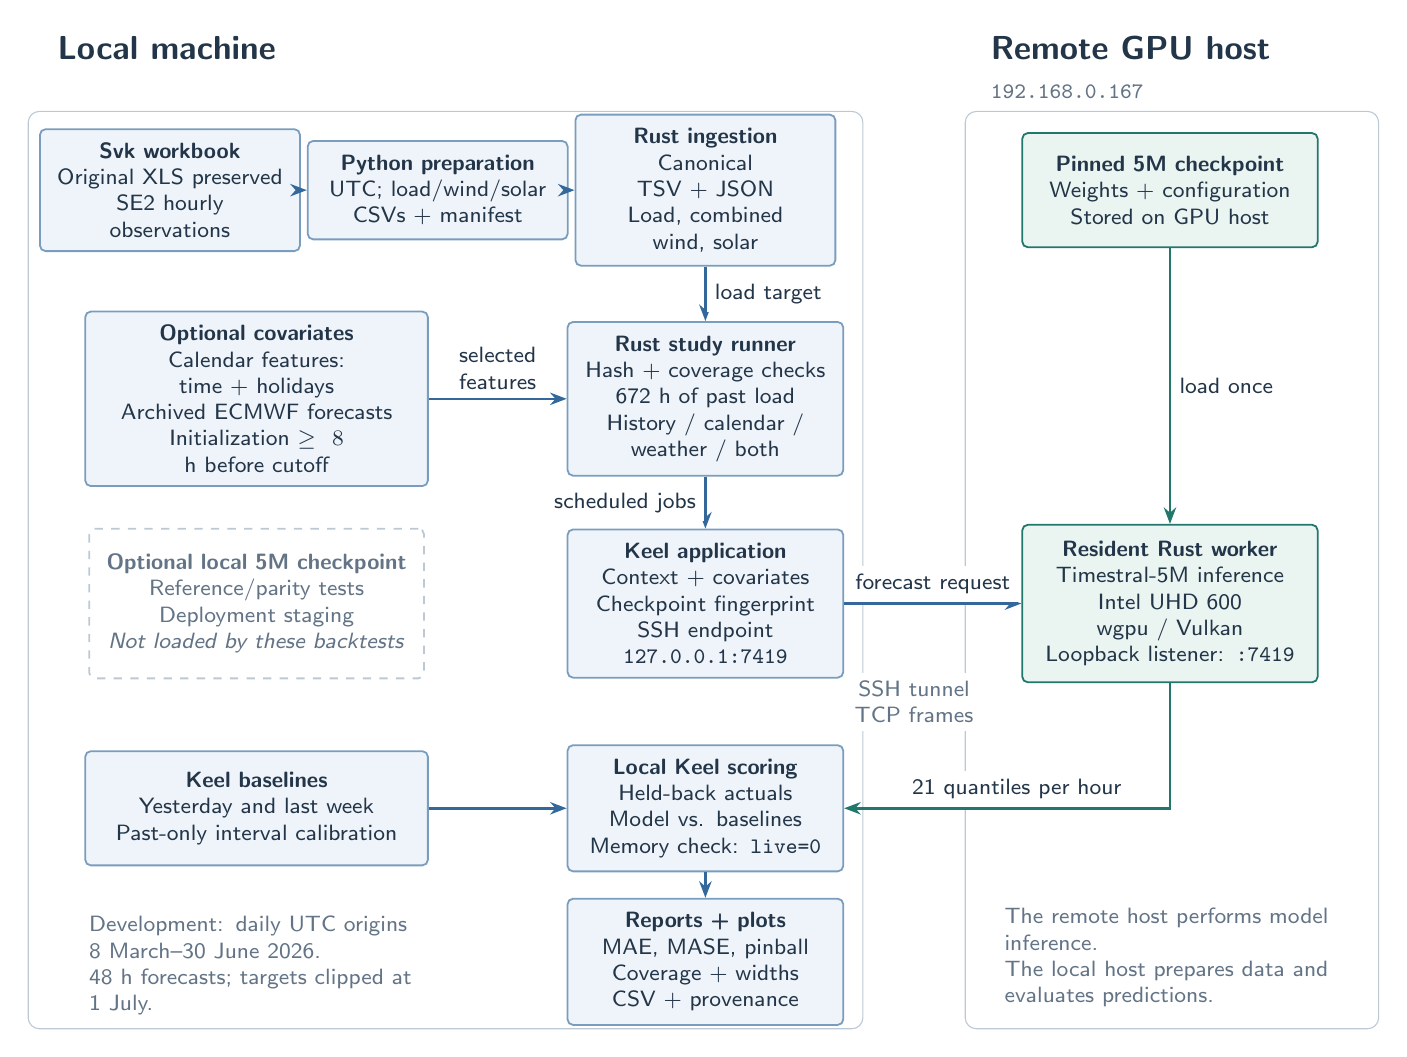
\begin{tikzpicture}[
  font=\sffamily\footnotesize, text=ink,
  box/.style={draw=blue!65,fill=paleBlue,rounded corners=2pt,
    line width=.65pt,align=center,text width=2.95cm,minimum height=1.25cm,inner sep=5pt},
  local/.style={box,text width=3.15cm},
  remote/.style={box,draw=teal,fill=paleTeal,text width=3.4cm},
  note/.style={box,draw=lightRule,dashed,fill=white,text=muted,text width=3.9cm},
  flow/.style={-{Stealth[length=2.1mm]},draw=blue,line width=.9pt},
  reply/.style={flow,draw=teal},
  edgeLabel/.style={font=\sffamily\footnotesize,align=center,fill=white,inner sep=3pt},
  heading/.style={font=\sffamily\bfseries\large,anchor=west}
]
% Execution boundaries. All preparation, orchestration and evaluation are local.
\draw[draw=lightRule,rounded corners=4pt] (-.25,1.0) rectangle (10.35,-10.65);
\draw[draw=lightRule,rounded corners=4pt] (11.65,1.0) rectangle (16.9,-10.65);
\node[heading] at (0,1.8) {Local machine};
\node[heading] at (11.85,1.8) {Remote GPU host};
\node[anchor=west,font=\sffamily\footnotesize,text=muted] at (11.85,1.25)
  {\texttt{192.168.0.167}};

% Preserved source, preparation and canonical data.
\node[box] (workbook) at (1.55,0) {\textbf{Svk workbook}\\Original XLS preserved\\SE2 hourly observations};
\node[box] (prepare) at (4.95,0) {\textbf{Python preparation}\\UTC; load/wind/solar\\CSVs + manifest};
\node[box] (canonical) at (8.35,0) {\textbf{Rust ingestion}\\Canonical TSV + JSON\\Load, combined wind, solar};
\draw[flow] (workbook) -- (prepare);
\draw[flow] (prepare) -- (canonical);

% The electricity target for these development runs is load. Wind and solar
% are imported for later ancillary use; they are not weather covariates.
\node[local,minimum height=1.8cm] (study) at (8.35,-2.65)
  {\textbf{Rust study runner}\\Hash + coverage checks\\672 h of past load\\History / calendar /\\weather / both};
\draw[flow] (canonical) -- node[edgeLabel,right] {load target} (study);
\node[box,text width=4cm,minimum height=1.7cm] (features) at (2.65,-2.65)
  {\textbf{Optional covariates}\\Calendar features: time + holidays\\Archived ECMWF forecasts\\Initialization $\geq 8$ h before cutoff};
\draw[flow] (features) -- node[edgeLabel,above] {selected\\features} (study);

% No runtime connection to the local weights: this copy is an offline asset.
\node[note,minimum height=1.9cm] (localweights) at (2.65,-5.25)
  {\textbf{Optional local 5M checkpoint}\\Reference/parity tests\\Deployment staging\\\emph{Not loaded by these backtests}};
\node[local,minimum height=1.5cm] (keel) at (8.35,-5.25)
  {\textbf{Keel application}\\Context + covariates\\Checkpoint fingerprint\\SSH endpoint\\\texttt{127.0.0.1:7419}};
\draw[flow] (study) -- node[edgeLabel,left] {scheduled jobs} (keel);

% The resident remote worker owns model loading and GPU computation.
\node[remote,minimum height=1.45cm] (weights) at (14.25,0)
  {\textbf{Pinned 5M checkpoint}\\Weights + configuration\\Stored on GPU host};
\node[remote,minimum height=2cm] (worker) at (14.25,-5.25)
  {\textbf{Resident Rust worker}\\Timestral-5M inference\\Intel UHD 600\\wgpu / Vulkan\\Loopback listener: \texttt{:7419}};
\draw[reply] (weights) -- node[edgeLabel,right] {load once} (worker);
\draw[flow] (keel.east) -- node[edgeLabel,above] {forecast request} (worker.west);
\node[edgeLabel,text=muted] at (11,-6.5)
  {SSH tunnel\\TCP frames};

% Local baselines and scoring use actuals only for evaluation, not as inputs.
\node[box,text width=4cm,minimum height=1.45cm] (baselines) at (2.65,-7.85)
  {\textbf{Keel baselines}\\Yesterday and last week\\Past-only interval calibration};
\node[local,minimum height=1.5cm] (score) at (8.35,-7.85)
  {\textbf{Local Keel scoring}\\Held-back actuals\\Model vs. baselines\\Memory check: \texttt{live=0}};
\draw[flow] (baselines) -- (score);
\draw[reply] (worker.south) -- (14.25,-7.85) --
  node[edgeLabel,above,pos=.47] {21 quantiles per hour} (score.east);
\node[local,minimum height=1.25cm] (reports) at (8.35,-9.8)
  {\textbf{Reports + plots}\\MAE, MASE, pinball\\Coverage + widths\\CSV + provenance};
\draw[flow] (score) -- (reports);
\node[align=left,text width=4.1cm,font=\sffamily\footnotesize,text=muted,anchor=west]
  at (.4,-9.85) {Development: daily UTC origins\\8 March--30 June 2026.\\48 h forecasts; targets clipped at 1 July.};
\node[align=left,text width=4.2cm,font=\sffamily\footnotesize,text=muted]
  at (14.25,-9.75) {The remote host performs model inference.\\The local host prepares data and evaluates predictions.};
\end{tikzpicture}
\end{document}
